% !TEX encoding = UTF-8 Unicode

\documentclass[12pt,a4j]{ltjsarticle}
\usepackage{semi}
\usepackage{here}

%\title{個人でのVR技術の利用状況} 
%\author{三原巧巳}
%\date{2022年12月14日} 
\begin{document} 

\begin{titlepage}
 \begin{center}
  
    \vspace*{20truept}
    
    {\LARGE 2023年度 卒業論文} 
    
    \vspace*{75truept}
    
    {\Huge } 個人でのVR技術の利用状況
    
    \vspace{85truept}
    
    {\LARGE 指導教員 須田 宇宙 准教授}
    
    \vspace{60truept}
    
    {\LARGE 千葉工業大学 情報ネットワーク学科}
    
    \vspace{15truept}
    
    {\LARGE 須田研究室}
    
    \vspace{70truept}
    
    {\LARGE 1931131 氏名 三原 巧巳 } % 氏名は消さない 学生番号 氏名 名前

    \vspace{70truept}
    
  \end{center}
  \begin{flushright}

    {\LARGE 提出日 2023年1月17日}
  
  \end{flushright}
\end{titlepage}

\setcounter{tocdepth}{3}
% 目次の出力
\tableofcontents
% 表目次
\listoftables
% 図目次
\listoffigures
\clearpage
\pagenumbering{arabic}
\setcounter{page}{1}

%\clearpage

%\tableofcontents
%\clearpage

\section{緒言}
近年,xR(AR,MR,VR)技術の発展により日常生活で技術の使用やコンテンツを見かけることが多くなった.
現在,xR技術は様々な形に変化して利用されている.
AR技術を利用するにはスマートフォンやスマートグラス,MR技術を利用するにはメガネや大きな機械のカメラなどで利用されている.
この2つの技術を用いたコンテンツは,広いスペースや大掛かりな設備を必要としない.

一方,VR技術を利用するには専用のヘッドマウントディスプレイを頭に着用し,視界の全体を覆った上で動き回るため,利用するコンテンツによっては大きな機材や広いスペースを必要とすることがある.
VR技術は主にゲームやアトラクション施設の場で利用されることが多いが,実際に利用できる施設や利用する場面が少ない.
利用される機会が少ないことで,VR技術の普及が低く技術の進化が起こらなくなる.
VR技術の進化がされないことで起こってしまうことは,エンターテイメントの幅が広がらないだけだはなく,現実で行うには危険な実習や現実では起こしにくい体験をすることが困難になるという問題がある.

本研究では,VR技術が普及しない理由として,現在あるVR技術のコンテンツにあると仮説を立て,それを元にVR機器の普及度と,購入されている種類・傾向,および購入していない人に対して購入していない理由などについて調査をし,普及率が低い原因を見つけることを目的としている.


\section{xR技術について}
\subsection{VR技術}
VRとは,「Virtual Reality」の略称であり「仮想現実」とも呼ばれている.
VR専用のヘッドマウントディスプレイやVRゴーグルを装着して,視界全体にコンピューターで作成した空間や世界の映像を映すことで自分が映像の中に入り込んだような体験ができる技術である.
さらにVRの中で自由な移動やものの操作などができ,現実に近い体験から非現実的な体験まで幅広くが扱うことができる.

VRコンテンツを利用するためには,専用のゴーグルが必要になりコンテンツによっては専用のコントローラーなども必要となる.
また体を動かすコンテンツの場合動かすのに十分な空間も必要となる.

VR技術では,主にゲームやエンターテイメントで普及してきたが,幅広い体験をできることから教育や訓練などでも利用されるようになり,近年ではビジネスの分野でも活躍するようになっっている.
ゲームやエンターテイメントの場では,専用のヘッドマウントディスプレイを利用したゲームの世界観を体験しながら遊べるコンテンツがある.
教育や訓練の場では,VRを利用した社会科見学や避難訓練の再現などといったもので利用されている.
ビジネスの場では,VRでの物件の内見やVRでのショッピングなどといったサービスが増えていっている.

VR技術のコンセプトは1935年ごろに作家のスタンリー・G・ワインボウムが発表したSF短編小説「Pygmalion’s Spectacles」の中に,ゴーグルを装着すると仮想的に五感を感じ取りながら擬似体験が可能な装置が登場する.
VR技術の研究が始まったのは1960年代頃かである.映画作成者で仮想現実技術のパイオニアであるモートン・ヘイリグが1962年にセンソラマと呼ばれる世界最初期のVR機器が開発された.
センソラマとは図\ref{fig:センソラマ.pdf}のような大型のシステムであり,没入型で多感覚入力が可能というマルチモーダルインターフェースを採用している.

\begin{figure}[h]
\begin{center}
 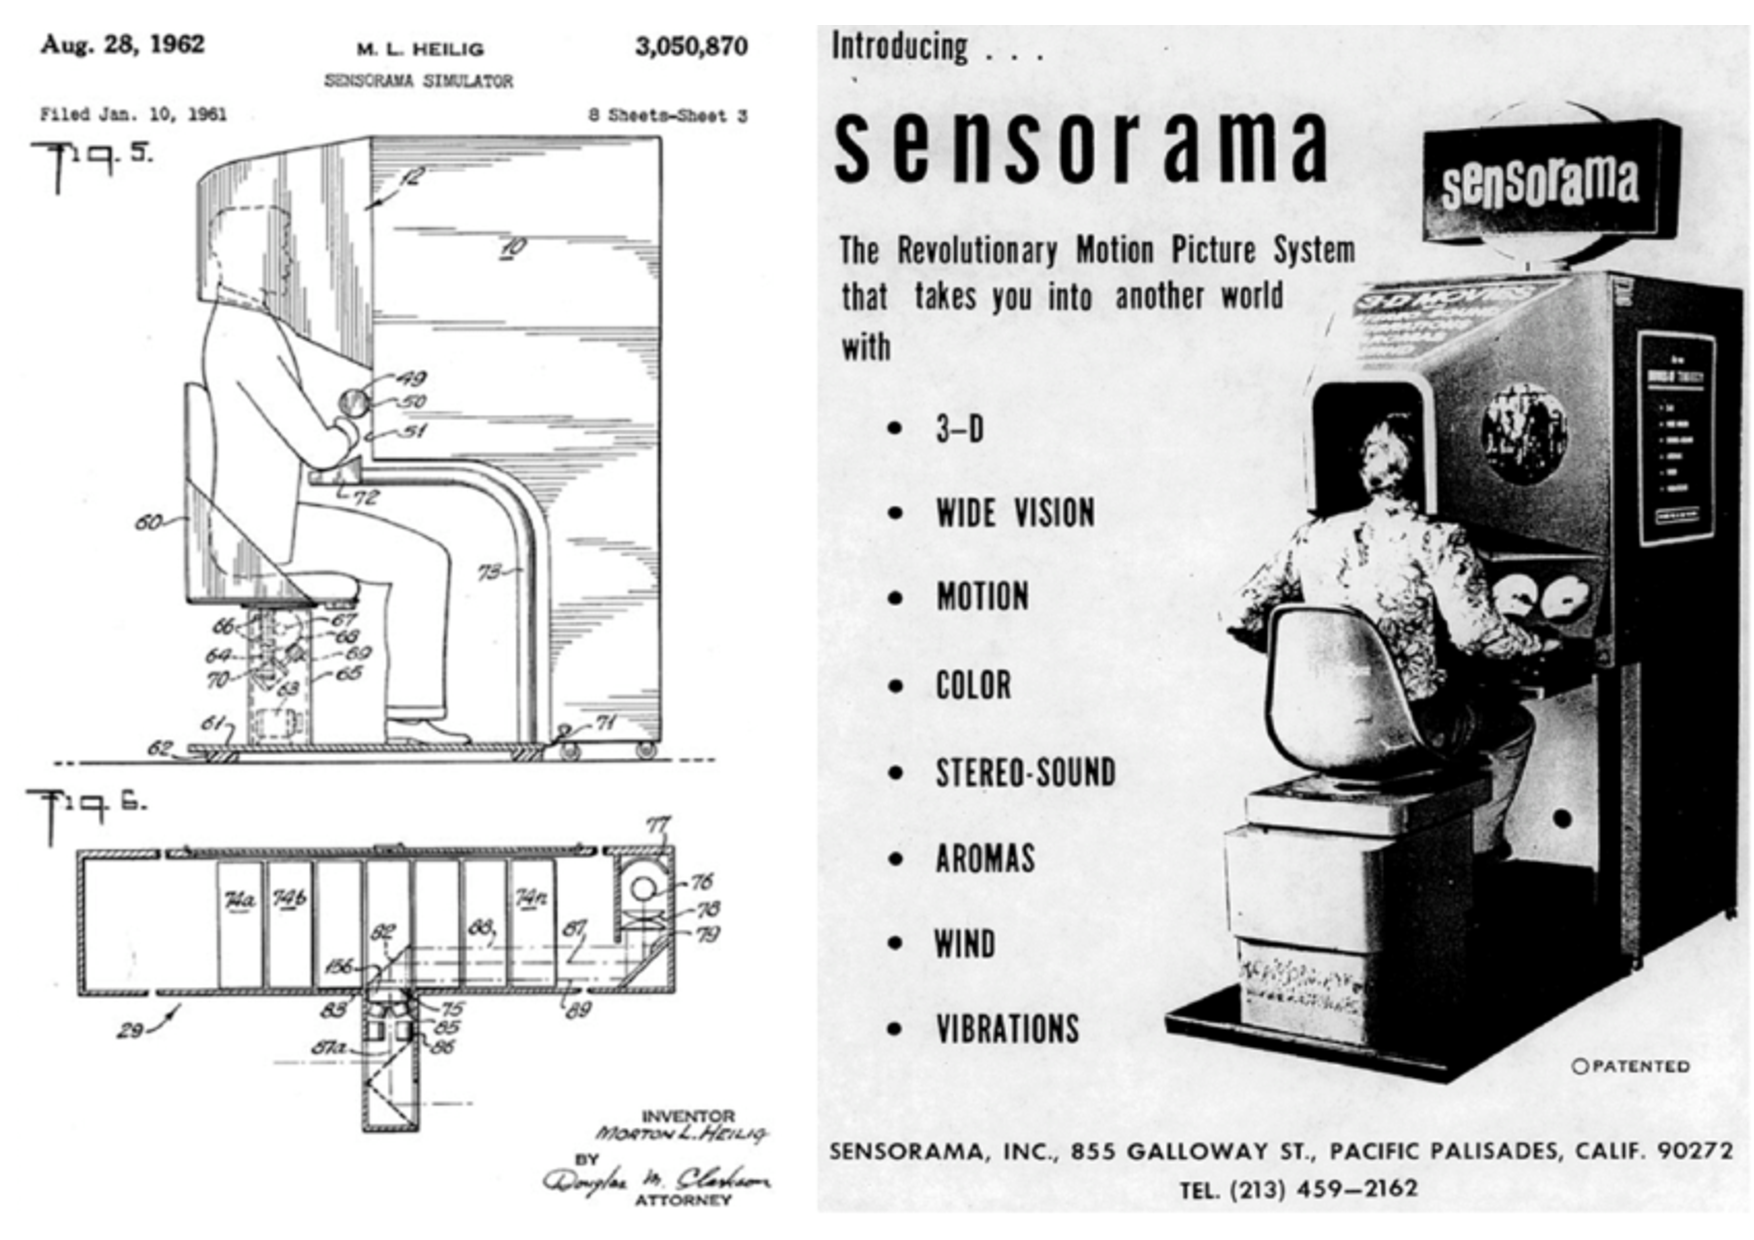
\includegraphics[clip,width=85mm,height=55mm]{センソラマ.pdf}
\end{center}
 \caption{センソラマ}
 \label{fig:センソラマ.pdf}
\end{figure}

その後1968年にユタ大学のアイバン・サザランドは,「ダモクレスの剣」というヘッドマウントディスプレイを開発したが,どちらも実用性が低くかった\cite{VRの概念の登場}.

1990年代前後からVR機器の商用化が始まった.
VPL Research社がRB2(Reality Built dfor 2)というVRを利用したコミュニケーションシステムを発表した.
このシステムは,ヘッドマウントディスプレイを使用した2人が同じVR空間で会話ができる3Dテレビ会議のようなシステムのようなシステムである.
しかし,当時のVR機器は価格が高いだけではなく性能が価格と見合っていないということから一般家庭に普及しなかった.
この商用化から約10年間はVRの第1次ブームと言われている\cite{VRの初の商用化}.

スマートフォンやゲーム機などのハードウェアの進化により2010年代以降にVRが再び注目される\cite{VRの概念の登場}.
スマートフォンでVRを利用したアプリケーションが開発されたり,以前より安価で性能が高くなった機器が出たことから,第1次ブームの時よりも日常的なものになろうとしている.

\subsection{AR技術}
ARとは,「Augmented Reality」の略称であり「拡張現実」とも呼ばれている.カメラで現実世界を映し,その上にCG映像や文字情報を重ねる技術である.
AR技術では,カメラを通して現実世界にポケモンや家具などのデジタルデータを映し出すことができる.
ARコンテンツを利用するためには,専用の機材を必要とせずスマートフォンやタブレットなどで利用することができる.

\subsection{MR技術}
MRとは,「Mixed Reality」の略称であり「複合現実」とも呼ばれいる.カメラを通して現実世界を認識し,実写とCG映像や文字情報を重ねることで現実世界と仮想世界を融合させる技術である.
主に医療や工業などで使われることが多く,車の設計や歯科治療のシミュレーションなどで普及している.
MR技術を利用するには,専用のデバイスやカメラだけではなく,仮想世界で作られたものを映すためのマーカーなども必要となる.

\section{xR機材について}
\subsection{VR機材}
\subsection{AR機材}
\subsection{MR機材}
\section{xRのコンテンツについて}
\subsection{VRのコンテンツ}
\subsection{ARのコンテンツ}
\subsection{MRのコンテンツ}
\section{第1回目のアンケート}
\subsection{仮説}
\subsection{内容}
\subsection{結果}
\section{第2回目のアンケート}
\subsection{仮説}
\subsection{内容}
\subsection{結果}
\section{考察}
\section{結言}
\section{謝辞}
\begin{thebibliography}{99}
\bibitem{VR}  ``流行体感から読み解くサービス未来予測 流行予想シリーズ ~VR(バーチャルリアリティ)編~'', https://research-platform.line.me/archives/38203466.html, 2022/9/2参照

\bibitem{VRの概念の登場}  ``VRはいつから普及が始まった?仮想現実の歴史を紐解く'', https://onetech.jp/blog/when-did-vr-become-popular-11526\#VR20, 2023/1/2参照

\bibitem{VRの初の商用化}  ``VRの初商用化は30年前、現代を生きるクリエイターが知っておくべき歴史と必要な視点とは'', https://creatorzine.jp/article/detail/538, 2023/1/2参照


\end{thebibliography}

\end{document}
